\documentclass[a4paper,12pt]{report}
\usepackage[T2A]{fontenc}
\usepackage[utf8]{inputenc}
\usepackage[english,russian]{babel}
\usepackage{graphicx}
\usepackage{wrapfig}
\usepackage{mathtext} 				% русские буквы в фомулах
\usepackage{amsmath,amsfonts,amssymb,amsthm,mathtools} % AMS
\usepackage{icomma} % "Умная" запятая: $0,2$ --- число, $0, 2$ --- перечисление
\usepackage{capt-of}
\usepackage{appendix}
\usepackage{multirow}
\usepackage{hyperref}
\usepackage{floatrow}
\usepackage[left=2cm,right=2cm,
    top=2cm,bottom=2cm,bindingoffset=0cm]{geometry}
\usepackage{multicol} % Несколько колонок
\usepackage{gensymb}
\title{Отчёт по лабораторной работе № 5.4.2. 

Исследование энергетического спектра $\beta$-спектра частиц и определение их максимальной энергии при помощи магнитного спектрометра.}
\author{Плюскова Н.А. Б04-004 }
\date{\today}
\begin{document}
\maketitle
\section*{1. Аннотация}
В данной работе были получены сила тока, соответствующая конверсионному пику, коэффициент пропорциональности, зависящий от параметров установки. Построен график Ферми-Кюри, по которому была найдена максимально возможная энергия электрона.

\section*{2. Теоретические сведения}
Бета-распадом называется самопроизвольное превращение ядер, при котором их массовое число не изменяется, а заряд увеличивается или уменьшается на единицу. Бета-активные ядра встречаются во всей области значений массового числа A, начиная от единицы (свободный нейтрон) и кончая самыми тяжелыми ядрами. Период полураспада $\beta$ - активных ядер изменяется от ничтожных долей секунды до $10^{18}$ лет. Выделяющаяся при единичном акте $\beta$ - распада энергия варьируется от 18 кэВ до 13,4 МэВ.

В данной работе мы будем иметь дело с электронным распадом

\begin{equation}\label{}
^A_ZX \rightarrow ^{\; \; \; \; \: A}_{Z+1}X + e^- + \widetilde{\nu}
\end{equation}

при котором кроме электрона испускается антинейтрино. Освобождающаяся при $\beta$-распаде энергия делится между электроном, антинейтрино и дочерним ядром, однако доля энергии, передаваемой ядру, исчезающе мала по сравнению с энергией, уносимой электроном и антинейтрино. Практически можно считать, что эти две частицы делят между собой всю освобождающуюся энергию. Поэтому электроны могут иметь любое значение энергии  от нулевой до некоторой максимальной, которая равна энергии, освобождающейся при $\beta$-распаде, являющейся важной физической величиной.

Вероятность $ dw $ того, что при распаде электрон вылетит с импульсом в интервале $d^3p$, а антинейтрино с импульсом в интервале $d^3k$, пропорциональна произведению этих дифференциалов. Но мы должны еще учесть закон сохранения энергии, согласно которому импульсы $ p $ и $ k $ электрона и антинейтрино связаны соотношением

\begin{equation}
E_e - E - ck = 0,
\end{equation}

где $E_e$ - максимальная энергия электрона, кинетическая энергия электрона $ E $ связана с его импульсом обычным релятивистским соотношением

\begin{equation}
E = c\sqrt{p^2 + m^2c^2} - mc^2,
\end{equation}

а через $ ck $ обозначена энергия антинейтрино с импульсом $ k $. Условие можно учесть введением в выражение для $ dw $ $\delta$ - функции
\begin{equation}
\delta (E_e - E - ck).
\end{equation}

Таким образом, вероятность $ dw $ может быть записана в виде

\begin{equation}\label{dw}
dw = D \delta (E_e - E - ck)d^3 p d^3 k = D \delta (E_e - E - ck)p^2dpk^2dkd{\Omega}_ed{\Omega}_{\widetilde{\nu}},
\end{equation}

где $ D $ --- некоторый коэффициент пропорциональности, $d\Omega_e$ , $d\Omega_{\widetilde{\nu}}$ --- элементы телесных углов направлений вылета электрона и нейтрино. Вероятность $ dw $ непосредственно связана с $\beta$-спектром, поскольку для большого числа $N_0$ распадов число $dN$ распадов с вылетом электрона и антинейтрино с импульсом соответственно от $ p $ до $ p + dp $ и от
$ k $ до $ k + d $k определяется соотношением

\begin{equation}\label{dn = n_0 dw}
dN = N_0 dw  
\end{equation}

Коэффициент $ D $ в формуле \eqref{dw} можно считать для рассматриваемых нами так называемых разрешенных фермиевских типов распадов с хорошей точностью константой (разрешенными называются такие переходы, при которых не изменяются ни момент, ни четность состояния ядра). В этом случае величину $ dw $ из \eqref{dn = n_0 dw} можно проинтегрировать по всем углам и по абсолютному значению импульса нейтрино.

После умножения на полное число распадов $ N $ проинтегрированное выражение приобретает смысл числа электронов $ dN $, вылетающих из ядра с импульсом, абсолютная величина которого лежит между $ p $ и$  p + dp $:

\begin{equation}\label{dN}
dN = \dfrac{16\pi^2 N_0}{c^2}Dp^2(E_e - E)^2dp.
\end{equation}

Чтобы получить распределение электронов по энергиям, надо в \eqref{dN} перейти от $ dp $ к $ dE $:

\begin{equation}
dE = \dfrac{c^2p}{E + mc^2}dp,
\end{equation}

после чего выражающая форму $\beta$ --- спектра величина $ N(E) = dN/dE $
приобретает вид

\begin{equation}\label{dN/dE big}
\dfrac{dN}{dE} = N_0Bcp(E + mc^2)(E_e - E)^2 = N_0B\sqrt{E(E + 2mc^2)}(E_e - E)^2(E + mc^2)
\end{equation}

где $B = (16\pi^2/c^4)D$. В нерелятивистском приближении, которое и имеет место с нашем случае, выражение \eqref{dN/dE big} упрощается, и мы имеем

\begin{equation}\label{dN/dE}
\dfrac{dN}{dE} \approx \sqrt{E}(E_e - E)^2.
\end{equation}

\begin{wrapfigure}[12]{l}{0.35\linewidth}
	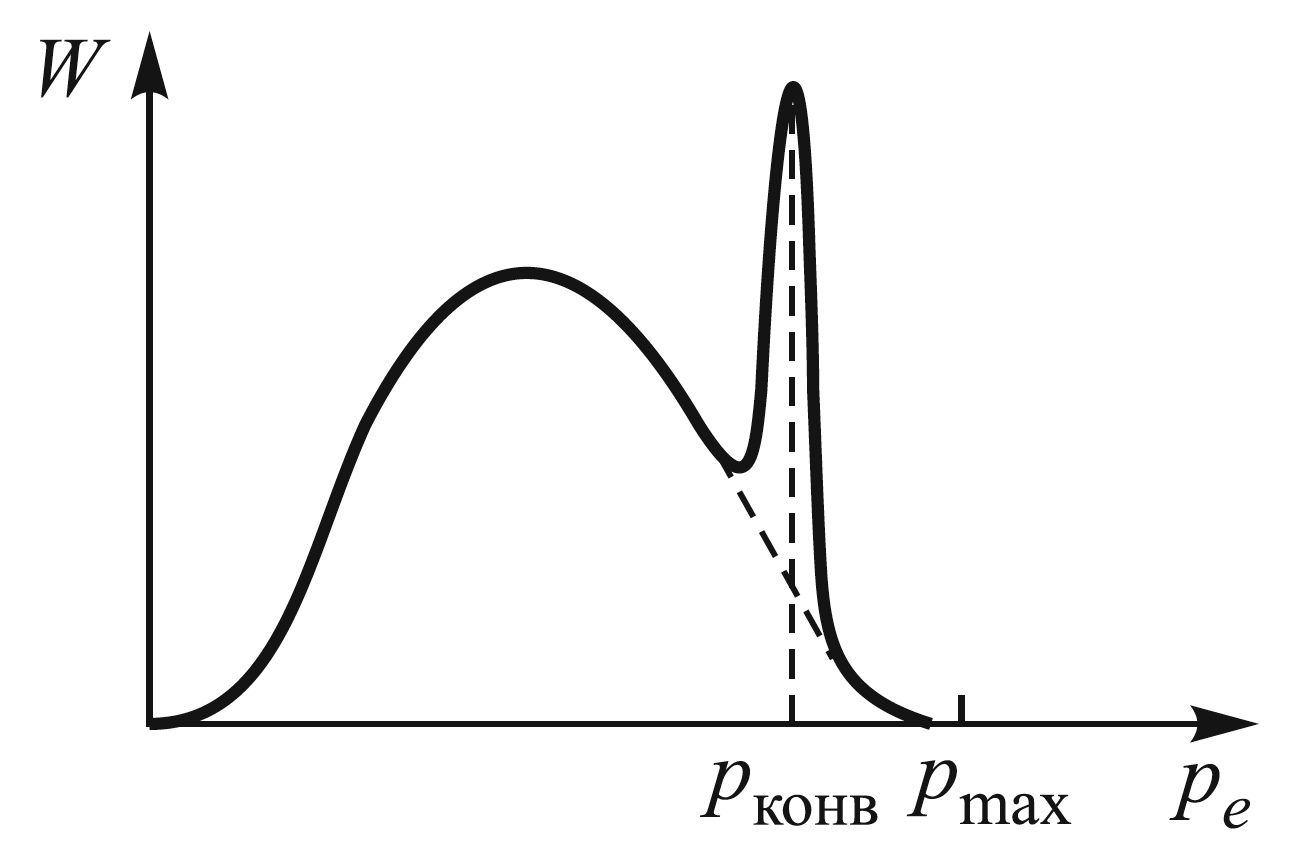
\includegraphics[width=\linewidth]{spektr}
	\caption{Форма спектра \be-частиц
		при разрешенных переходах}
	\label{ris spetr}
\end{wrapfigure}


Выражение \eqref{dN/dE} приводит к спектру, имеющему вид широкого колокола (рис \ref{ris spetr}). Кривая плавно отходит от нуля и столь же плавно, по параболе, касается оси абсцисс в области максимальной энергии электронов $E_e$. 

Дочерние ядра, возникающие в результате $\beta$-распада, нередко оказываются возбужденными. Возбужденные ядра отдают свою энергию либо излучая $\gamma$-квант (энергия которого равна разности энергий начального и конечного уровней), либо передавая избыток энергии одному из электронов с внутренних оболочек атома. Излучаемые в таком процессе электроны имеют строго определенную энергию и называются конверсионными.

Конверсия чаще всего происходит на оболочках $ K $ или $ L $. На спектре, представленном на рис. \ref{ris spetr}, видна монохроматическая линия, вызванная электронами конверсии. Ширина этой линии в нашем случае является чисто аппаратурной, по ней можно оценить разрешающую силу спектрометра.


\section*{3. Экспериментальная установка}
Для определения энергии $\beta$-частиц в работе используется магнитный спектрометр, схема которого показана на рисунке \ref{pic:scheme} слева. Электроны испускаются радиоактивным источником и попадают в магнитное поле катушки, ось которой параллельна $OZ$. Траектории электронов сходятся в одной точке --- фокусе, где и установлен сцинтилляционный счетчик, сигналы которого усиливаются фотоумножителем и регистрируются пересчетным прибором. Фокусное расстояние $f$ магнитной линзы связано с током в катушке $I$ и импульсом $p_e$ регистрируемых частиц следующим образом:
	
	\[ \frac{1}{f} \propto \frac{I^2}{p_e^2} \]  
	
	При неизменной геометрии установки, увеличивая и уменьшая силу тока, можно фокусировать электроны разных импульсов, причем 
	
	\begin{equation}\label{k}
	p_e = kI,
	\end{equation}
	
	 где $k$ --- коэффициент пропорциональности, являющийся параметром установки.

	\begin{figure}[h]
	\centering
	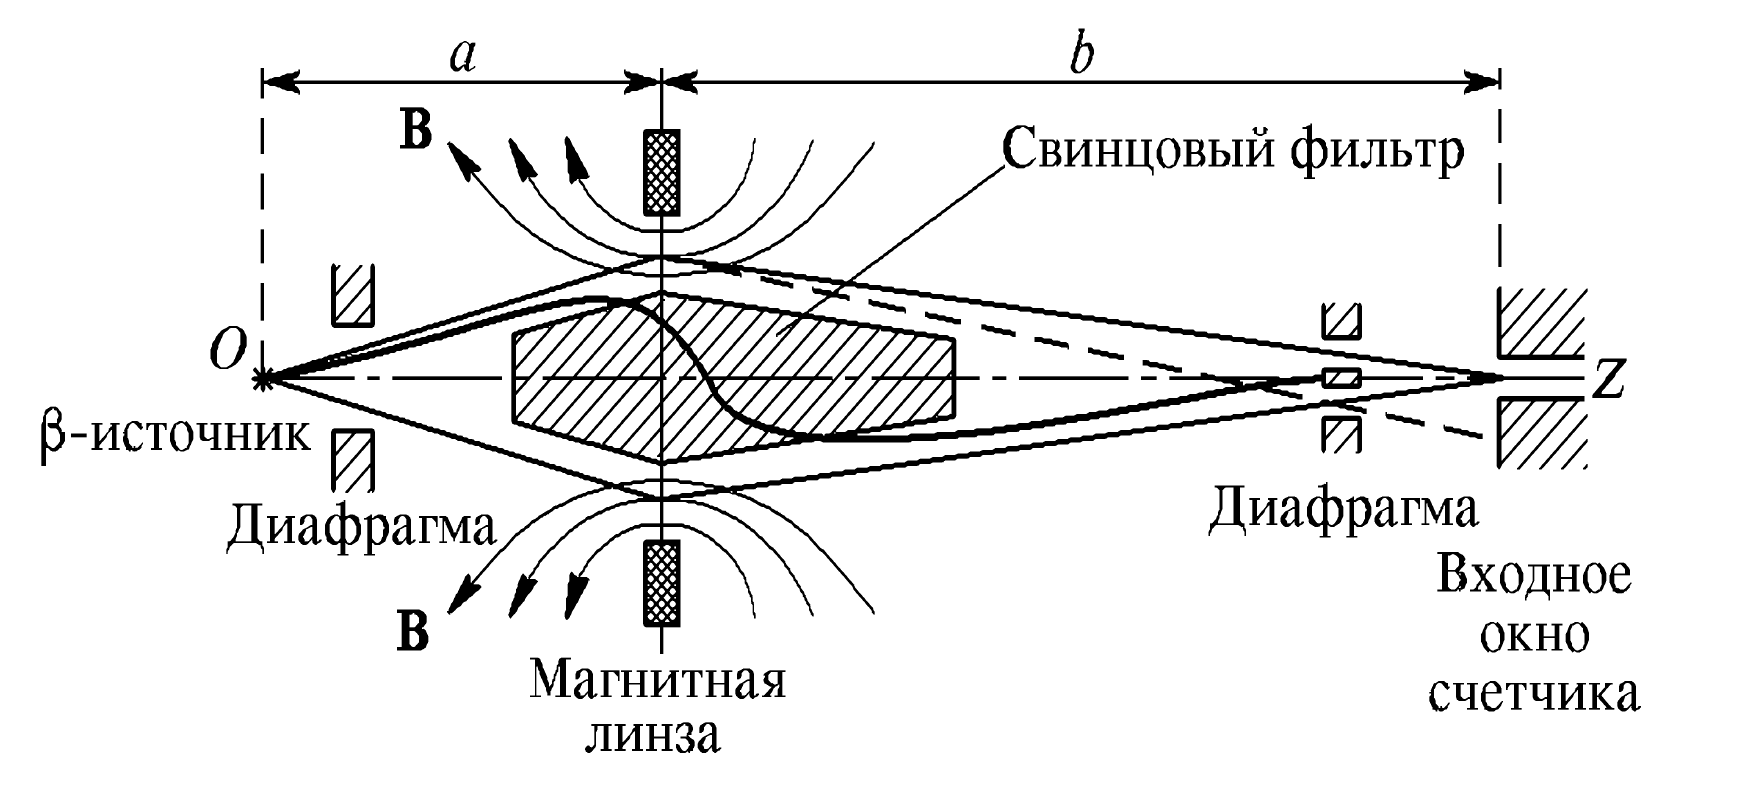
\includegraphics[width=0.48\textwidth]{lab}
	\hfill
	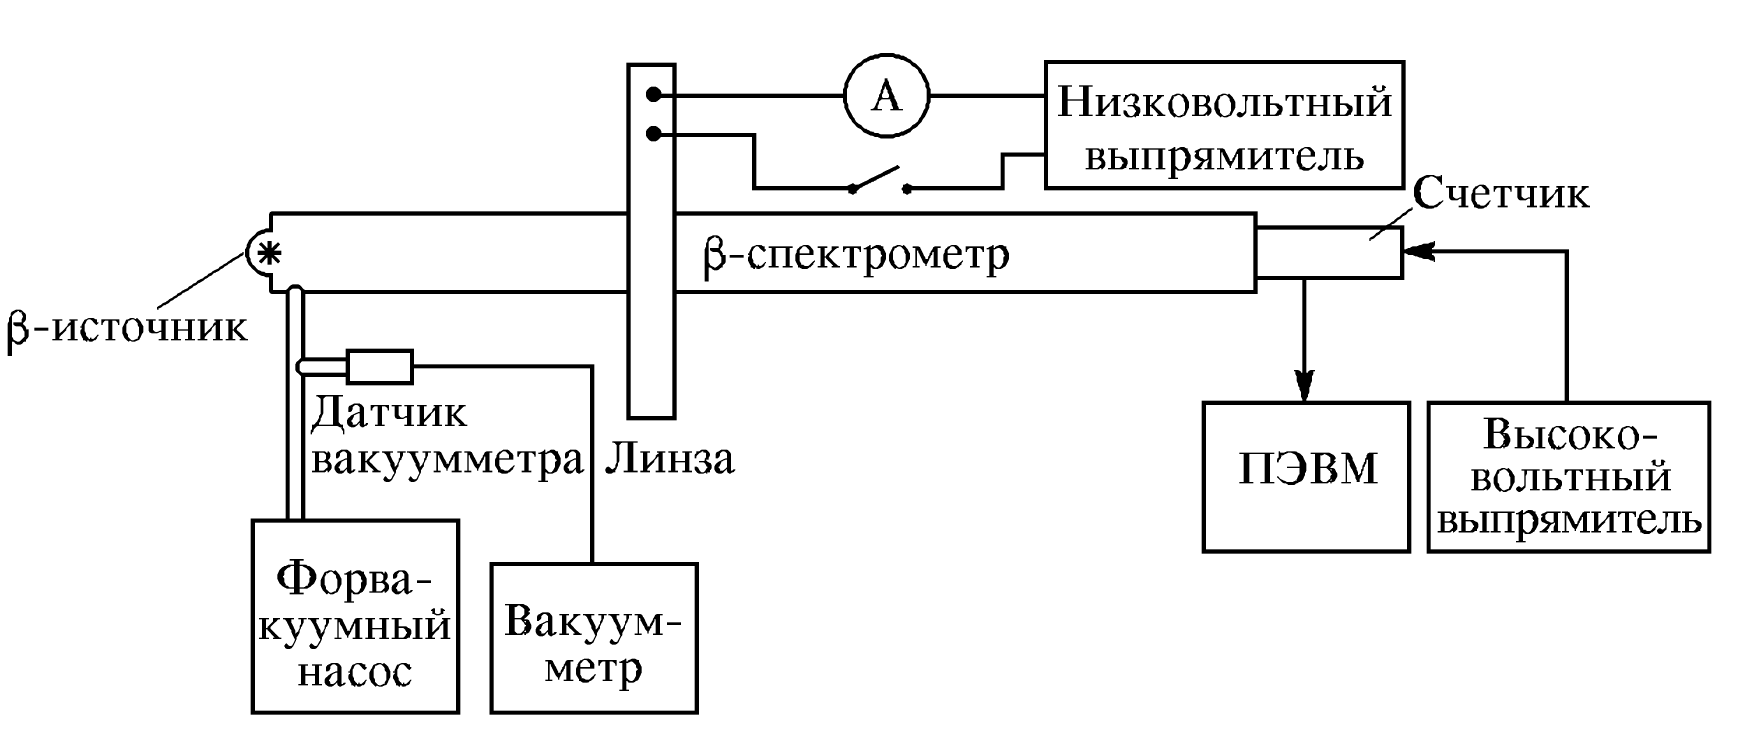
\includegraphics[width=0.48\textwidth]{lab2}
	\caption{слева --- схема $\beta$-спектрометра; справа --- блок-схема установки для изучения спектра}
	\label{pic:scheme}
\end{figure}

В $\beta$-спектрометре установлены диафрагмы для ограничения углов вылета частиц из источника и свинцовый фильтр для защиты от прямого попадания $\gamma$-лучей. 

Число частиц $N$, регистрируемых на установке, равно: $N \approx W \cdot \Delta p_e$, где $\Delta p_e$ - разрешающая способность спектрометра. Дифференцируя выражение для форуса магнитной линзы, получим: $\Delta p_e = \frac{1}{2}\frac{\Delta f}{f}p_e$, то есть $\Delta p_e \propto p_e$. Таким образом, для количества частиц справедлива формула: 

\begin{equation}\label{N}
 N = CW(p_e)p_e 
\end{equation}

Здесь $C$ - некоторая константа.
\section*{4. Ход работы}
Проведем измерения $\beta$-спектра, изменяя ток $I$ магнитной линзы:

\begin{table}[H]
\begin{tabular}{|c|c|c|c|}
\hline
$I$, А & $\sigma_{I}$, А              & $N, c^{-1}$ & $\sigma_{N},c^{-1}$ \\ \hline
0,20 & \multirow{24}{*}{0,01} & 0,860        & 0,093             \\ \cline{1-1} \cline{3-4} 
0,40 &                        & 0,960        & 0,098             \\ \cline{1-1} \cline{3-4} 
0,60 &                        & 0,770        & 0,088             \\ \cline{1-1} \cline{3-4} 
0,80 &                        & 1,040        & 0,102             \\ \cline{1-1} \cline{3-4} 
1,00 &                        & 1,380        & 0,117             \\ \cline{1-1} \cline{3-4} 
1,10 &                        & 1,560        & 0,125             \\ \cline{1-1} \cline{3-4} 
1,20 &                        & 2,049        & 0,143             \\ \cline{1-1} \cline{3-4} 
1,30 &                        & 2,489        & 0,158             \\ \cline{1-1} \cline{3-4} 
1,40 &                        & 2,669        & 0,163             \\ \cline{1-1} \cline{3-4} 
1,50 &                        & 3,099        & 0,176             \\ \cline{1-1} \cline{3-4} 
1,60 &                        & 3,149        & 0,177             \\ \cline{1-1} \cline{3-4} 
1,70 &                        & 3,189        & 0,179             \\ \cline{1-1} \cline{3-4} 
1,80 &                        & 3,959        & 0,199             \\ \cline{1-1} \cline{3-4} 
1,90 &                        & 3,699        & 0,192             \\ \cline{1-1} \cline{3-4} 
2,00 &                        & 4,069        & 0,202             \\ \cline{1-1} \cline{3-4} 
2,10 &                        & 4,449        & 0,211             \\ \cline{1-1} \cline{3-4} 
2,20 &                        & 4,489        & 0,212             \\ \cline{1-1} \cline{3-4} 
2,30 &                        & 4,399        & 0,210             \\ \cline{1-1} \cline{3-4} 
2,40 &                        & 4,449        & 0,211             \\ \cline{1-1} \cline{3-4} 
2,50 &                        & 4,189        & 0,205             \\ \cline{1-1} \cline{3-4} 
2,60 &                        & 4,419        & 0,210             \\ \cline{1-1} \cline{3-4} 
2,70 &                        & 4,029        & 0,201             \\ \cline{1-1} \cline{3-4} 
2,80 &                        & 4,029        & 0,201             \\ \cline{1-1} \cline{3-4} 
2,90 &                        & 3,649        & 0,191             \\ \hline
\end{tabular}
\hspace{1cm}
\begin{tabular}{|c|c|c|c|}
\hline
$I$, А & $\sigma_{I}$, А              & $N, c^{-1}$ & $\sigma_{N},c^{-1}$ \\ \hline
3,00 & \multirow{24}{*}{0,01} & 3,449        & 0,186             \\ \cline{1-1} \cline{3-4} 
3,10 &                        & 3,109        & 0,176             \\ \cline{1-1} \cline{3-4} 
3,20 &                        & 2,559        & 0,160             \\ \cline{1-1} \cline{3-4} 
3,30 &                        & 2,119        & 0,146             \\ \cline{1-1} \cline{3-4} 
3,40 &                        & 1,809        & 0,134             \\ \cline{1-1} \cline{3-4} 
3,50 &                        & 1,410        & 0,119             \\ \cline{1-1} \cline{3-4} 
3,60 &                        & 1,180        & 0,109             \\ \cline{1-1} \cline{3-4} 
3,70 &                        & 1,090        & 0,104             \\ \cline{1-1} \cline{3-4} 
3,80 &                        & 1,759        & 0,133             \\ \cline{1-1} \cline{3-4} 
3,85 &                        & 2,659        & 0,163             \\ \cline{1-1} \cline{3-4} 
3,90 &                        & 3,379        & 0,184             \\ \cline{1-1} \cline{3-4} 
3,95 &                        & 4,189        & 0,205             \\ \cline{1-1} \cline{3-4} 
4,00 &                        & 4,369        & 0,209             \\ \cline{1-1} \cline{3-4} 
4,05 &                        & 4,988        & 0,223             \\ \cline{1-1} \cline{3-4} 
4,10 &                        & 6,828        & 0,261             \\ \cline{1-1} \cline{3-4} 
4,15 &                        & 6,368        & 0,252             \\ \cline{1-1} \cline{3-4} 
4,20 &                        & 5,698        & 0,239             \\ \cline{1-1} \cline{3-4} 
4,25 &                        & 5,548        & 0,236             \\ \cline{1-1} \cline{3-4} 
4,30 &                        & 5,388        & 0,232             \\ \cline{1-1} \cline{3-4} 
4,32 &                        & 4,359        & 0,209             \\ \cline{1-1} \cline{3-4} 
4,35 &                        & 3,129        & 0,177             \\ \cline{1-1} \cline{3-4} 
4,40 &                        & 2,279        & 0,151             \\ \cline{1-1} \cline{3-4} 
4,45 &                        & 1,480        & 0,122             \\ \cline{1-1} \cline{3-4} 
4,50 &                        & 0,970        & 0,098             \\ \hline
\end{tabular}
\caption{Измерение $\beta$-спектра}
\end{table}

Также измерим фон, чтобы в дальнейших рассуждениях учесть его:

\begin{table}[H]
\begin{tabular}{|c|c|c|c|c|}
\hline
$I$, А & $\sigma_{I}$, А              & $N, c^{-1}$ & $\sigma_{N},c^{-1}$ & $t$, c \\ \hline
0    & \multirow{2}{*}{0,01} & 0,707        & 0,049             & 300  \\ \cline{1-1} \cline{3-5} 
5,98 &                       & 0,403        & 0,037             & 300  \\ \hline
\end{tabular}
\caption{Измерение фона}
\end{table}

Построим график $N(I)$, с помощью которого прокалибруем спектрометр:

	\begin{figure}[H]
		\centering
		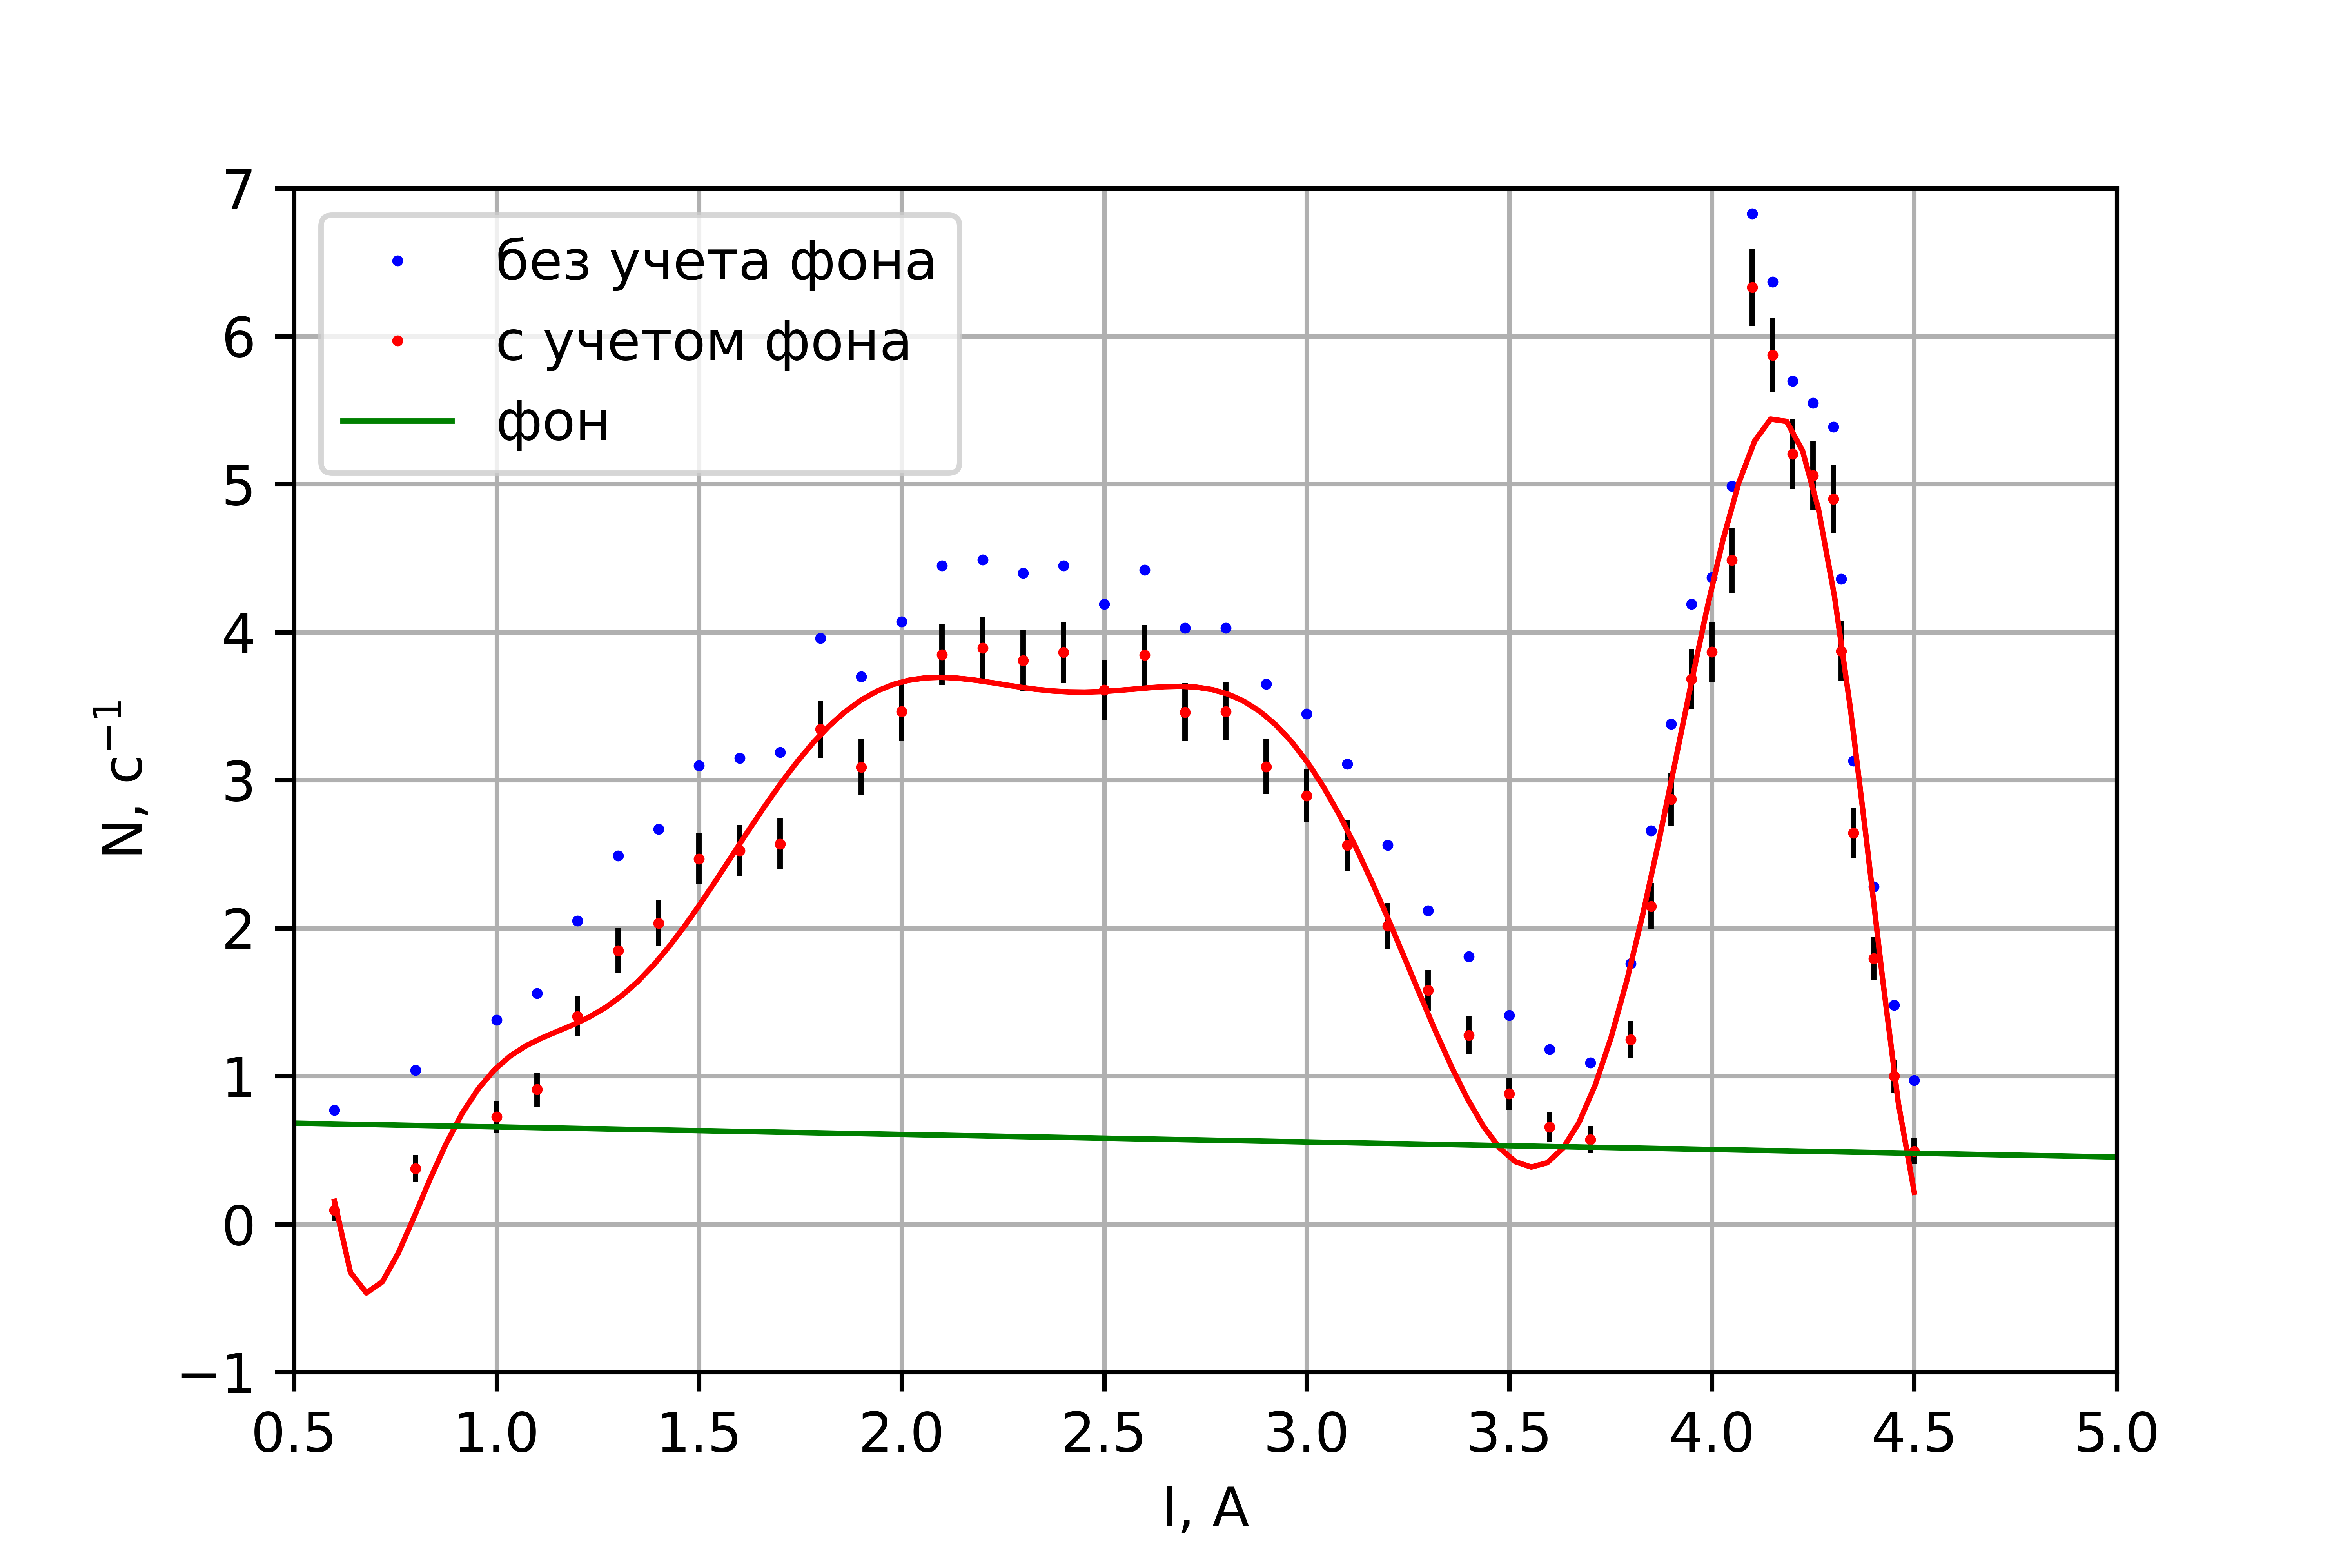
\includegraphics[width=0.7\linewidth]{N(I).png}
		\caption{$N(I)$}
		\label{ris mu}
	\end{figure}

График $N(I)$ аппроксимируем полиномом 10 степени. По уравнению аппроксимирующей кривой находим величину силы тока, соответствующую конверсионному пику: $I = (4,16 \pm 0,04)$ А

Отсюда находим константу $k$,являющуюся параметром установки:
\begin{equation*}
    k = \frac{pc}{I} = (244\pm 2) \text{ кэВ/А}
\end{equation*}

Построим график Ферми-Кюри:

	\begin{figure}[H]
		\centering
		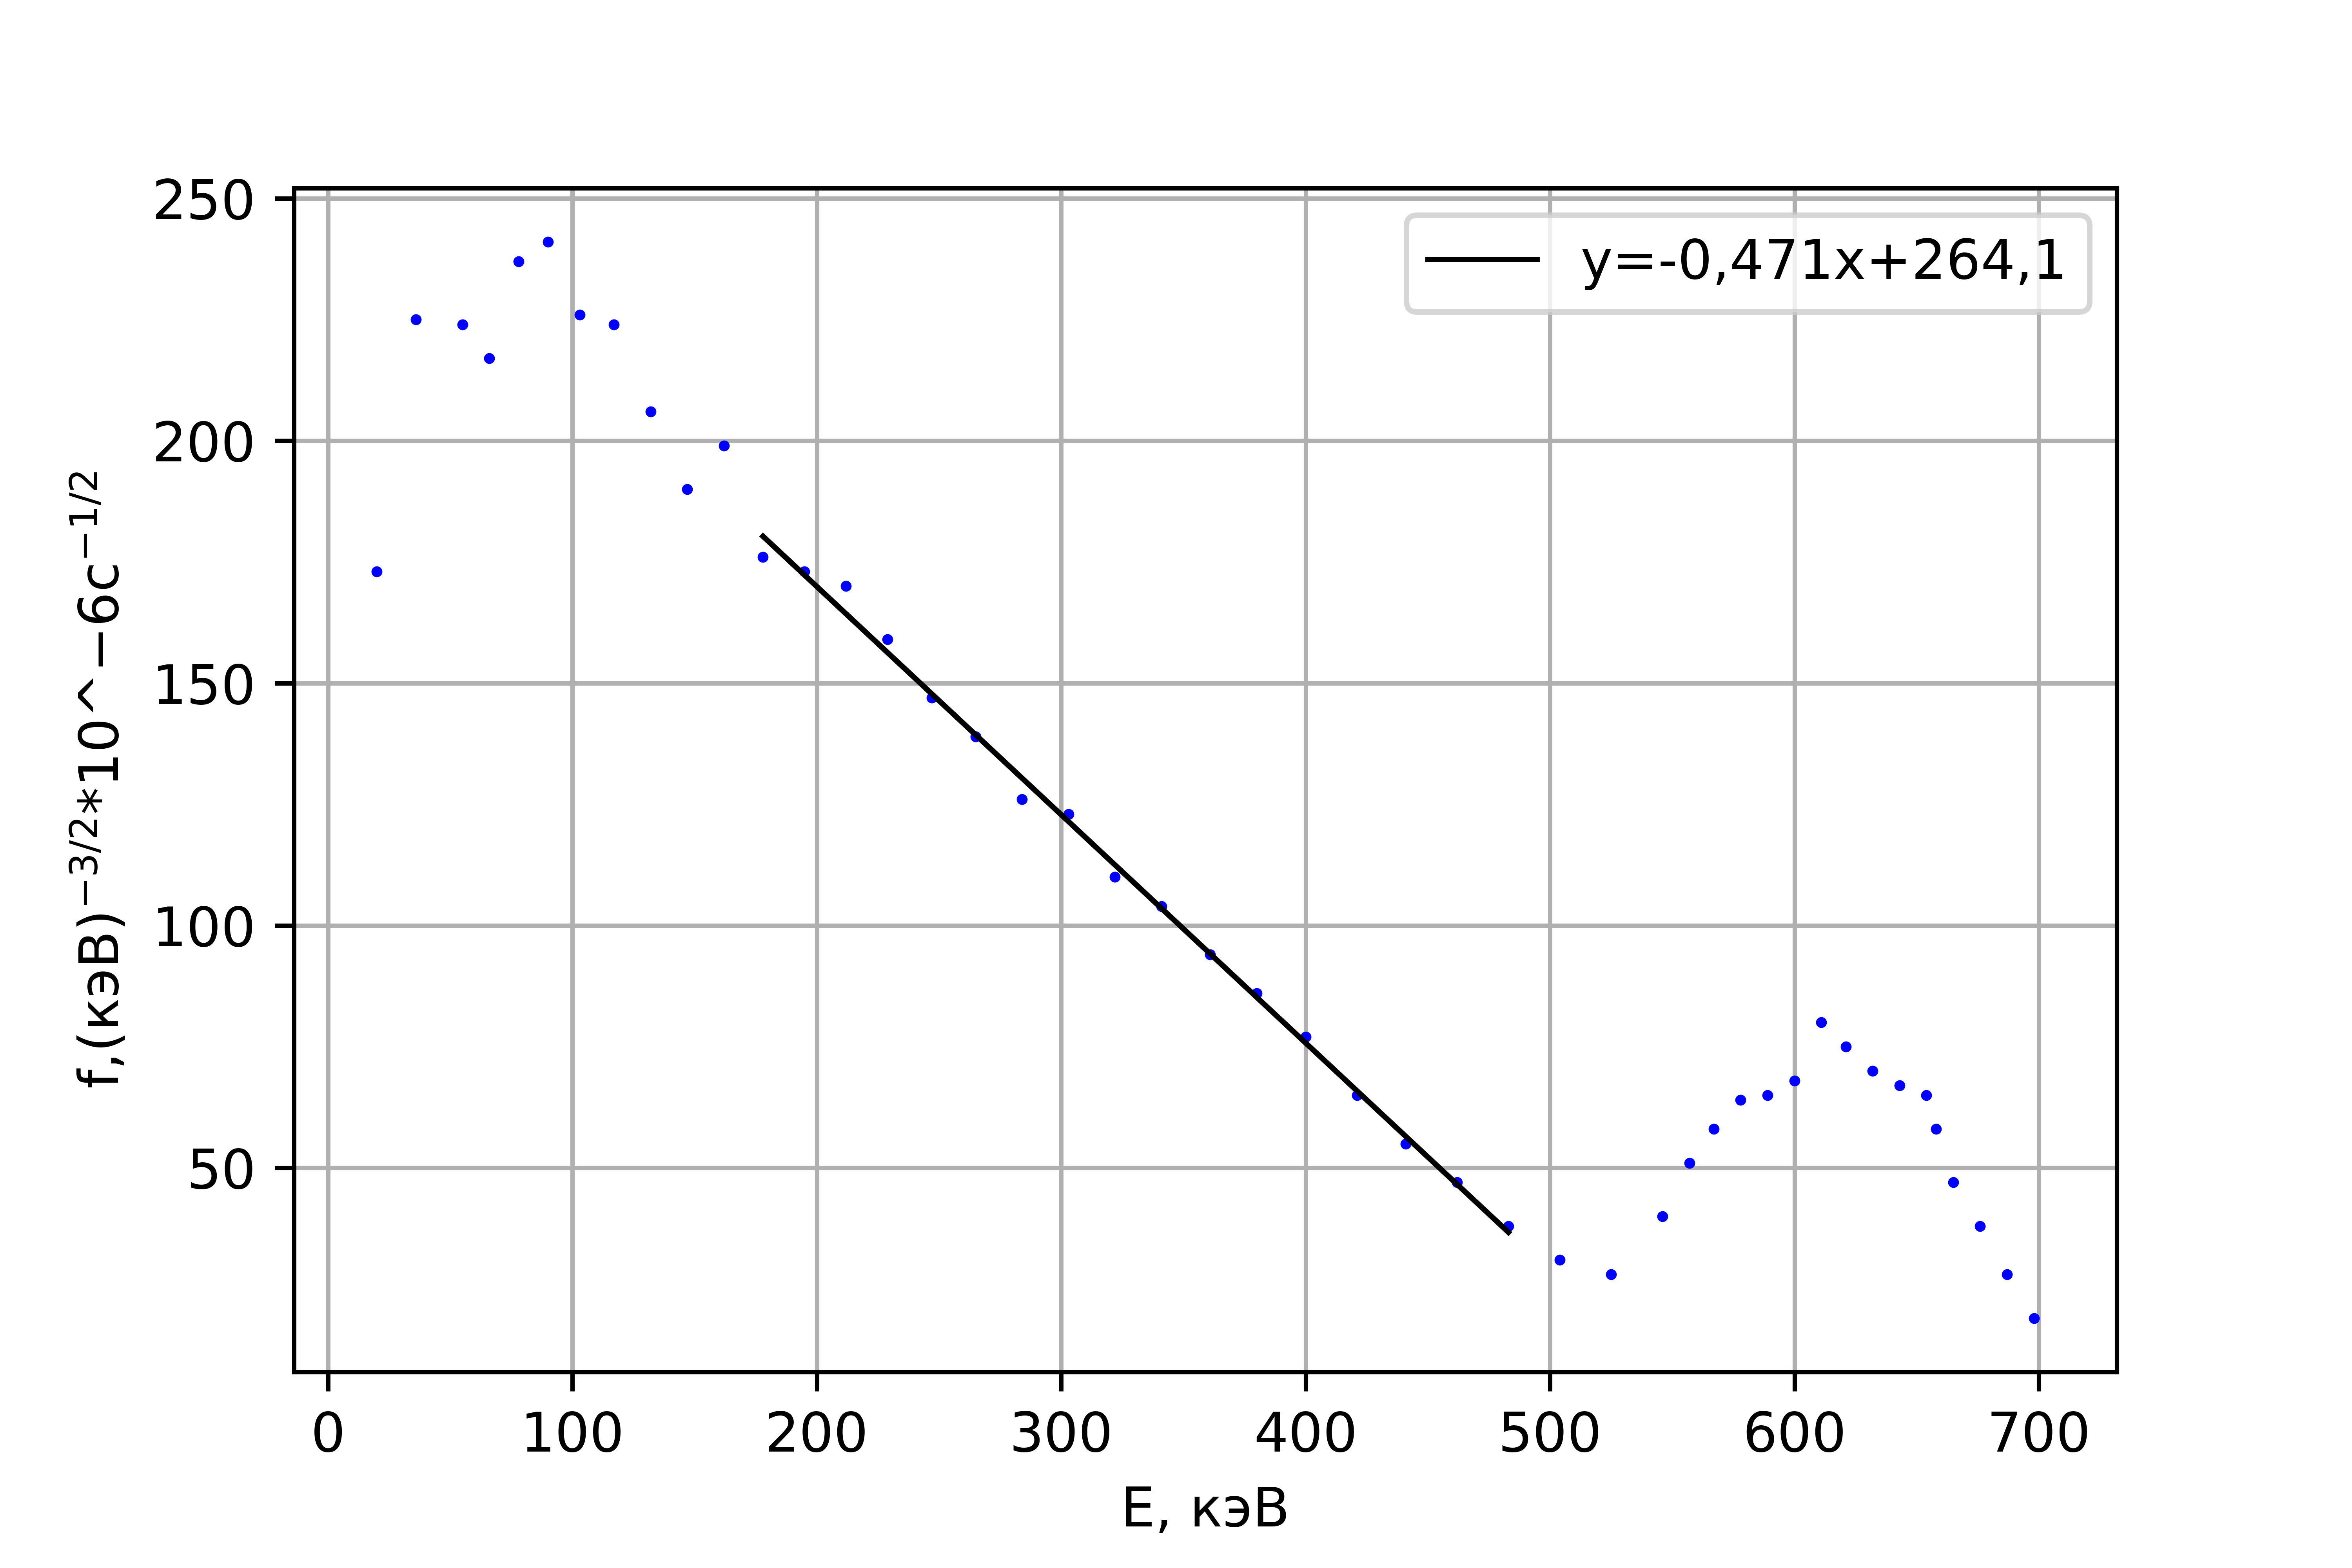
\includegraphics[width=0.7\linewidth]{f(E).png}
		\caption{$\frac{\sqrt{N(p)}}{p}(E)$}
		\label{ris mu}
	\end{figure}

Из графика находим максимальную энергию электронов, как пересечение аппроксимирующей прямой с осью абсцисс: $E_{e} = \frac{-b}{a} = (561\pm3) $ кэВ. (Погрешность $\sigma_{E_{e}}$ нашли из МНК)

\begin{table}[H]
\begin{tabular}{|c|c|c|c|c|c|}
\hline
$N,   c^{-1}$ & $\sigma_{N}, c^{-1}$ & $\frac{p}{c}$,кэВ & $\sigma_{\frac{p}{c}}$,кэВ & $\frac{\sqrt{N-N_{bg}}}{p^{3/2}}*10^{-6}$, кэВ^{-3/2}*c^{-1/2}  & $E$, кэВ \\ \hline
0,770          & 0,088             & 146,4    & 12,2           & 173                                     & 20     \\ \hline
1,040          & 0,102             & 195,2    & 16,2           & 225                                     & 36     \\ \hline
1,380          & 0,117             & 244,0    & 20,1           & 224                                     & 55     \\ \hline
1,560          & 0,125             & 268,4    & 22,1           & 217                                     & 66     \\ \hline
2,049          & 0,143             & 292,8    & 24,1           & 237                                     & 78     \\ \hline
2,489          & 0,158             & 317,2    & 26,1           & 241                                     & 90     \\ \hline
2,669          & 0,163             & 341,6    & 28,1           & 226                                     & 103    \\ \hline
3,099          & 0,176             & 366,0    & 30,1           & 224                                     & 117    \\ \hline
3,149          & 0,177             & 390,4    & 32,1           & 206                                     & 132    \\ \hline
3,189          & 0,179             & 414,8    & 34,1           & 190                                     & 147    \\ \hline
3,959          & 0,199             & 439,2    & 36,1           & 199                                     & 162    \\ \hline
3,699          & 0,192             & 463,6    & 38,1           & 176                                     & 178    \\ \hline
4,069          & 0,202             & 488,0    & 40,1           & 173                                     & 195    \\ \hline
4,449          & 0,211             & 512,4    & 42,1           & 170                                     & 212    \\ \hline
4,489          & 0,212             & 536,8    & 44,1           & 159                                     & 229    \\ \hline
4,399          & 0,210             & 561,2    & 46,1           & 147                                     & 247    \\ \hline
4,449          & 0,211             & 585,6    & 48,1           & 139                                     & 265    \\ \hline
4,189          & 0,205             & 610,0    & 50,1           & 126                                     & 284    \\ \hline
4,419          & 0,210             & 634,4    & 52,1           & 123                                     & 303    \\ \hline
4,029          & 0,201             & 658,8    & 54,1           & 110                                     & 322    \\ \hline
4,029          & 0,201             & 683,2    & 56,1           & 104                                     & 341    \\ \hline
3,649          & 0,191             & 707,6    & 58,0           & 94                                      & 361    \\ \hline
3,449          & 0,186             & 732,0    & 60,0    & 86                                      & 380    \\ \hline
3,109          & 0,176             & 756,4    & 62,0    & 77                                      & 400    \\ \hline
2,559          & 0,160             & 780,8    & 64,0    & 65                                      & 421    \\ \hline
2,119          & 0,146             & 805,2    & 66,0    & 55                                      & 441    \\ \hline
1,809          & 0,134             & 829,6    & 68,0    & 47                                      & 462    \\ \hline
1,410          & 0,119             & 854,0    & 70,0    & 38                                      & 483    \\ \hline
1,180          & 0,109             & 878,4    & 72,0    & 31                                      & 504    \\ \hline
1,090          & 0,104             & 902,8    & 74,0    & 28                                      & 525    \\ \hline
1,759          & 0,133             & 927,2    & 76,0    & 40                                      & 546    \\ \hline
2,659          & 0,163             & 939,4    & 77,0    & 51                                      & 557    \\ \hline
3,379          & 0,184             & 951,6    & 78,0    & 58                                      & 567    \\ \hline
4,189          & 0,205             & 963,8    & 79,0    & 64                                      & 578    \\ \hline
4,369          & 0,209             & 976,0    & 80,0    & 65                                      & 589    \\ \hline
4,988          & 0,223             & 988,2    & 81,0    & 68                                      & 600    \\ \hline
6,828          & 0,261             & 1000,4   & 82,0    & 80                                      & 611    \\ \hline
6,368          & 0,252             & 1012,6   & 83,0    & 75                                      & 621    \\ \hline
5,698          & 0,239             & 1024,8   & 84,0    & 70                                      & 632    \\ \hline
5,548          & 0,236             & 1037,0   & 85,0    & 67                                      & 643    \\ \hline
5,388          & 0,232             & 1049,2   & 86,0    & 65                                      & 654    \\ \hline
4,359          & 0,209             & 1054,1   & 86,4    & 58                                      & 658    \\ \hline
3,129          & 0,177             & 1061,4   & 87,0    & 47                                      & 665    \\ \hline
2,279          & 0,151             & 1073,6   & 88,0    & 38                                      & 676    \\ \hline
1,480          & 0,122             & 1085,8   & 89,0    & 28                                      & 687    \\ \hline
0,970          & 0,098             & 1098,0   & 90,0    & 19                                      & 698    \\ \hline
\end{tabular}
\caption{Данные для построения графика Ферми-Кюри}
\end{table}

\section*{5. Выводы}
В работе был изучен спектр $\beta$-распада $  ^{136} Cs $, получены значение тока для конверсионного пика $I = (4,16 \pm 0,04)$ А, $k$ - коэффициент пропорциональности, являющийся параметром установки $k= (244\pm 2) \text{ кэВ/А}$, а также максимально возможная энергия электрона $E_{e}  = (561\pm3) $ кэВ


\end{document}
